% !TEX TS-program = xelatex
% !TEX encoding = UTF-8 Unicode
\documentclass[aspectratio=169,10pt]{beamer}

% Template base: standard Beamer structure (e.g., Overleaf "Beamer presentation").
\usetheme{Madrid}
\usecolortheme{default}
\setbeamertemplate{navigation symbols}{}
\setbeamertemplate{caption}[numbered]

\usepackage{iftex}
\ifPDFTeX
  \usepackage[utf8]{inputenc}
  \usepackage[T1]{fontenc}
  \usepackage{lmodern}
\else
  \usepackage{fontspec}
  % Keep fonts conservative for MiKTeX portability.
  \setsansfont{Latin Modern Sans}
  \setmainfont{Latin Modern Roman}
  \setmonofont{Latin Modern Mono}
\fi

\usepackage{microtype}
\usepackage{etoolbox}
\usepackage{graphicx}
\usepackage{booktabs}
\usepackage{amsmath}
\usepackage{amssymb}
\usepackage{xurl}
\usepackage{tikz}
\usetikzlibrary{arrows.meta,positioning,calc}

% beamer already loads hyperref; configure it here.
\hypersetup{hidelinks}

% Bibliography (same pipeline as main.tex: xelatex -> biber -> xelatex)
\usepackage[backend=biber,style=ieee]{biblatex}
\addbibresource{references.bib}
\setcounter{biburlnumpenalty}{100}
\setcounter{biburlucpenalty}{100}
\setcounter{biburllcpenalty}{100}

\graphicspath{{figures/}{assets/}}

% Avoid empty bibliography warning when no citations are used.
\newif\ifhascites
\hascitesfalse
\AtBeginDocument{%
  \pretocmd{\cite}{\global\hascitestrue}{}{}%
  \pretocmd{\parencite}{\global\hascitestrue}{}{}%
  \pretocmd{\textcite}{\global\hascitestrue}{}{}%
  \pretocmd{\footcite}{\global\hascitestrue}{}{}%
  \pretocmd{\autocite}{\global\hascitestrue}{}{}%
}

% Metadata
\title[Midterm -- Nhận dạng]{Báo cáo giữa kỳ: Phát hiện khuôn mặt\\từ Viola--Jones đến SCRFD (ICLR 2022)}
\author[Nhóm 23KHMT]{23127333 Trương Quốc Cường \and 23127011 Lê Anh Duy \and 23127199 Trần Gia Huy}
\institute[HCMUS]{CSC14006 -- Nhận dạng\\Trường ĐH Khoa học Tự nhiên, ĐHQG-HCM}
\date[HK2 2025--2026]{Học kỳ 2 -- Năm học 2025--2026}
\titlegraphic{
\includegraphics[height=0.9cm]{HCMUS.png}}

\begin{document}

\begin{frame}
  \titlepage
\end{frame}

\begin{frame}{Mục lục}
  \tableofcontents
\end{frame}

\section{Bối cảnh và tiêu chí}

\begin{frame}{Thông tin đề tài}
  \begin{itemize}
    \setlength{\itemsep}{4pt}
    \item \textbf{Chương sách (Chương I):} \textit{Face Detection} trong \textit{Handbook of Face Recognition} (2nd ed.), Chapter 11.\ \cite{li2012facechapter}
    \item \textbf{Bài báo (Chương II):} \textit{Sample and Computation Redistribution for Efficient Face Detection} (SCRFD), ICLR 2022.\ \cite{guo2022scrfd}
    \item \textbf{Mục tiêu giữa kỳ:} nắm khung phát hiện 3 bước; tái lập Viola--Jones (minh họa OpenCV); phân tích SCRFD theo paper.
  \end{itemize}
\end{frame}

\begin{frame}{Tiêu chí chấm điểm (6 mục)}
  \small
  \setlength{\tabcolsep}{5pt}
  \renewcommand{\arraystretch}{1.15}
  \begin{tabular}{@{}p{0.72\textwidth}cc@{}}
    \toprule
    \textbf{Tiêu chí} & \textbf{Max} & \textbf{Chương} \\
    \midrule
    1. Nhận dạng \& mô tả kỹ thuật trong chương sách & 2.0 & I \\
    2. Phân tích phương pháp trong bài báo khoa học & 2.0 & II \\
    3. Mối liên hệ giữa chương sách và bài báo & 2.0 & II \\
    4. Điểm mạnh, hạn chế, phạm vi áp dụng & 2.0 & I + II \\
    5. Nhận định cá nhân \& khả năng mở rộng & 1.0 & II \\
    6. Trình bày học thuật \& liêm chính (trích dẫn) & 1.0 & Tất cả \\
    \bottomrule
  \end{tabular}
\end{frame}

\section{Chương I -- Kỹ thuật trong chương sách (cổ điển)}

\begin{frame}{(1) Kỹ thuật trung tâm của chương sách}
  \begin{block}{Kỹ thuật cốt lõi}
    Khung phát hiện khuôn mặt đa tỉ lệ kiểu \textbf{Viola--Jones}: tháp ảnh + quét cửa sổ trượt + chấm điểm nhanh bằng Haar/Integral Image + \textbf{cascade} tăng cường (AdaBoost).\ \cite{li2012facechapter,viola2001rapid,viola2004robust}
  \end{block}
  \begin{itemize}
    \setlength{\itemsep}{4pt}
    \item \textbf{Mục tiêu:} phát hiện thời gian thực trên ảnh tĩnh/video (tối ưu tốc độ, giảm báo động giả).
    \item \textbf{Đặc điểm bài toán:} số lượng cửa sổ âm \(\gg\) dương \(\Rightarrow\) loại sớm là chiến lược then chốt.
  \end{itemize}
\end{frame}

\begin{frame}{Khung phát hiện 3 bước (tư duy hệ thống)}
  \begin{enumerate}
    \setlength{\itemsep}{6pt}
    \item \textbf{Sinh giả thuyết (proposal generation):} tháp ảnh + cửa sổ trượt tạo ra tập ứng viên ở nhiều tỉ lệ.
    \item \textbf{Chấm điểm / phân loại:} đánh giá nhanh từng cửa sổ (weak-to-strong).
    \item \textbf{Hợp nhất kết quả:} ngưỡng hóa + Non-Maximum Suppression (NMS).
  \end{enumerate}
  \vspace{6pt}
  \begin{center}
    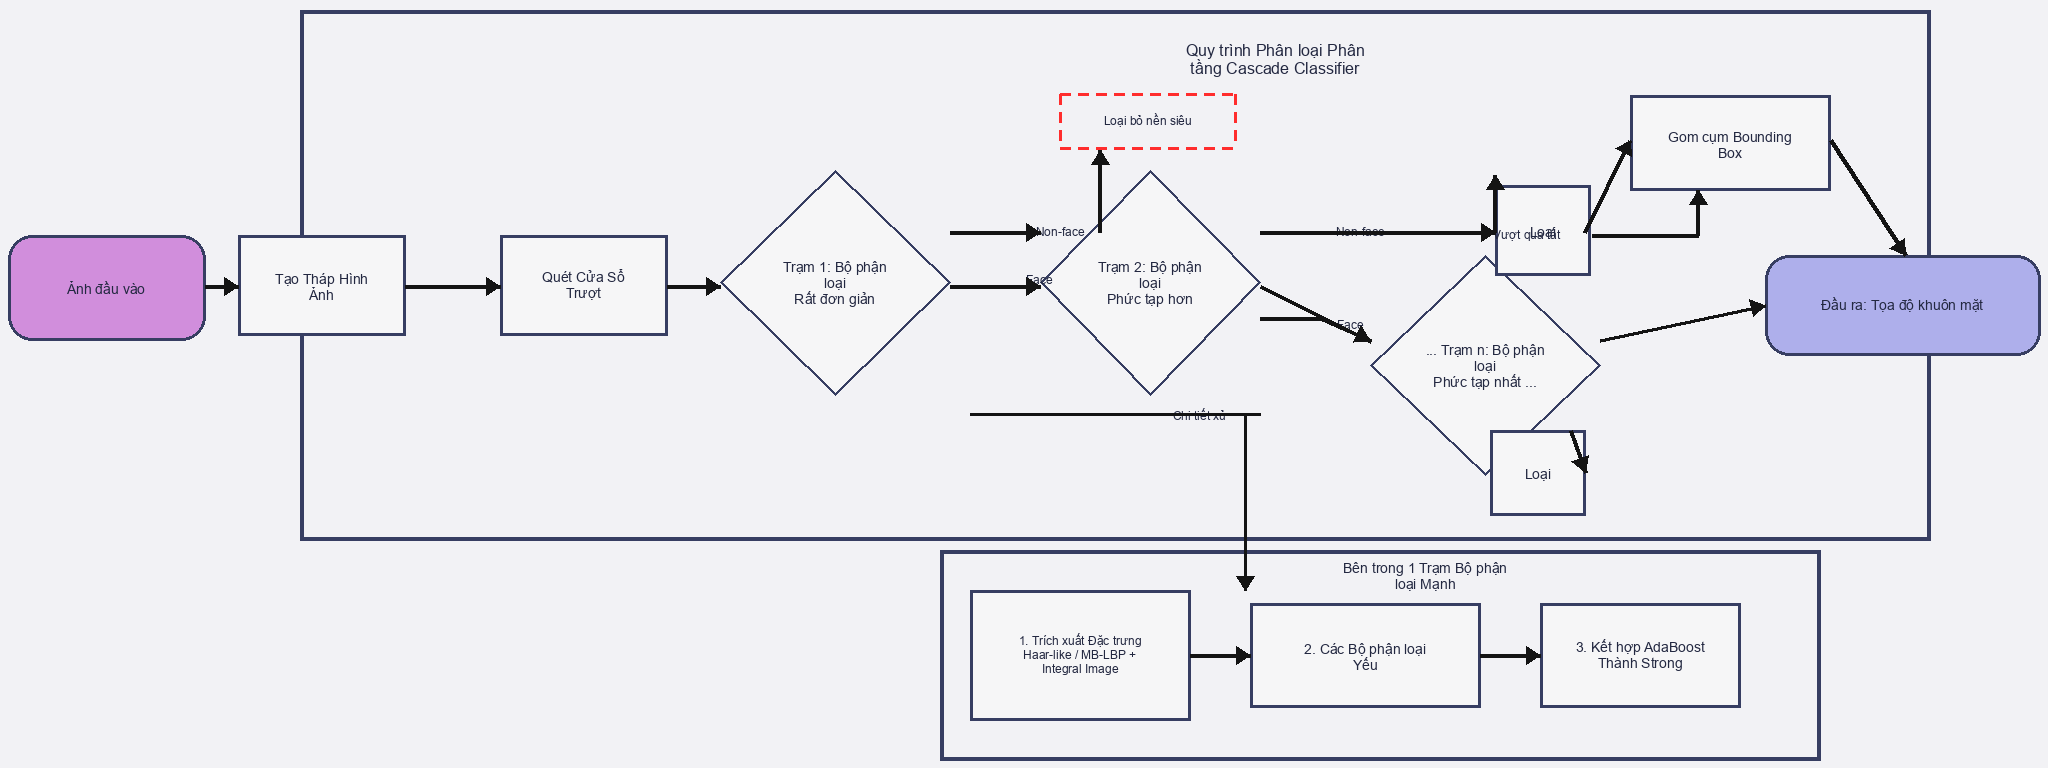
\includegraphics[width=0.92\linewidth]{custom/classical_cascade_detailed_flow.png}
  \end{center}
\end{frame}

\begin{frame}{Integral Image và đặc trưng Haar-like (mô hình toán)}
  \begin{block}{Integral Image}
    \[
      I_{\Sigma}(x,y) = \sum_{x'\le x,\,y'\le y} I(x',y')
    \]
    Tổng cường độ trong một hình chữ nhật bất kỳ tính trong \(O(1)\) phép toán (4 truy vấn) \(\Rightarrow\) trích xuất Haar-like rất nhanh.\ \cite{viola2001rapid,viola2004robust}
  \end{block}
  \begin{itemize}
    \setlength{\itemsep}{4pt}
    \item \textbf{Haar-like:} hiệu giữa các vùng sáng/tối (mắt--má, sống mũi--hai bên, \ldots).
    \item \textbf{Hệ quả:} số đặc trưng khả dĩ cực lớn \(\Rightarrow\) cần cơ chế chọn lọc tự động (AdaBoost).
  \end{itemize}
\end{frame}

\begin{frame}{AdaBoost và Cascade classifier (nguyên lý vận hành)}
  \begin{itemize}
    \setlength{\itemsep}{5pt}
    \item \textbf{AdaBoost:} chọn đặc trưng phân biệt + kết hợp weak learners \(\Rightarrow\) strong classifier.\ \cite{viola2001rapid}
    \item \textbf{Cascade:} nhiều ``trạm'' tăng dần độ mạnh; nếu trượt ngưỡng ở trạm sớm thì loại ngay.
    \item \textbf{Ưu tiên tốc độ:} phần lớn cửa sổ âm dừng ở trạm rất sớm \(\Rightarrow\) gần thời gian thực.
  \end{itemize}
  \vspace{6pt}
  \begin{center}
    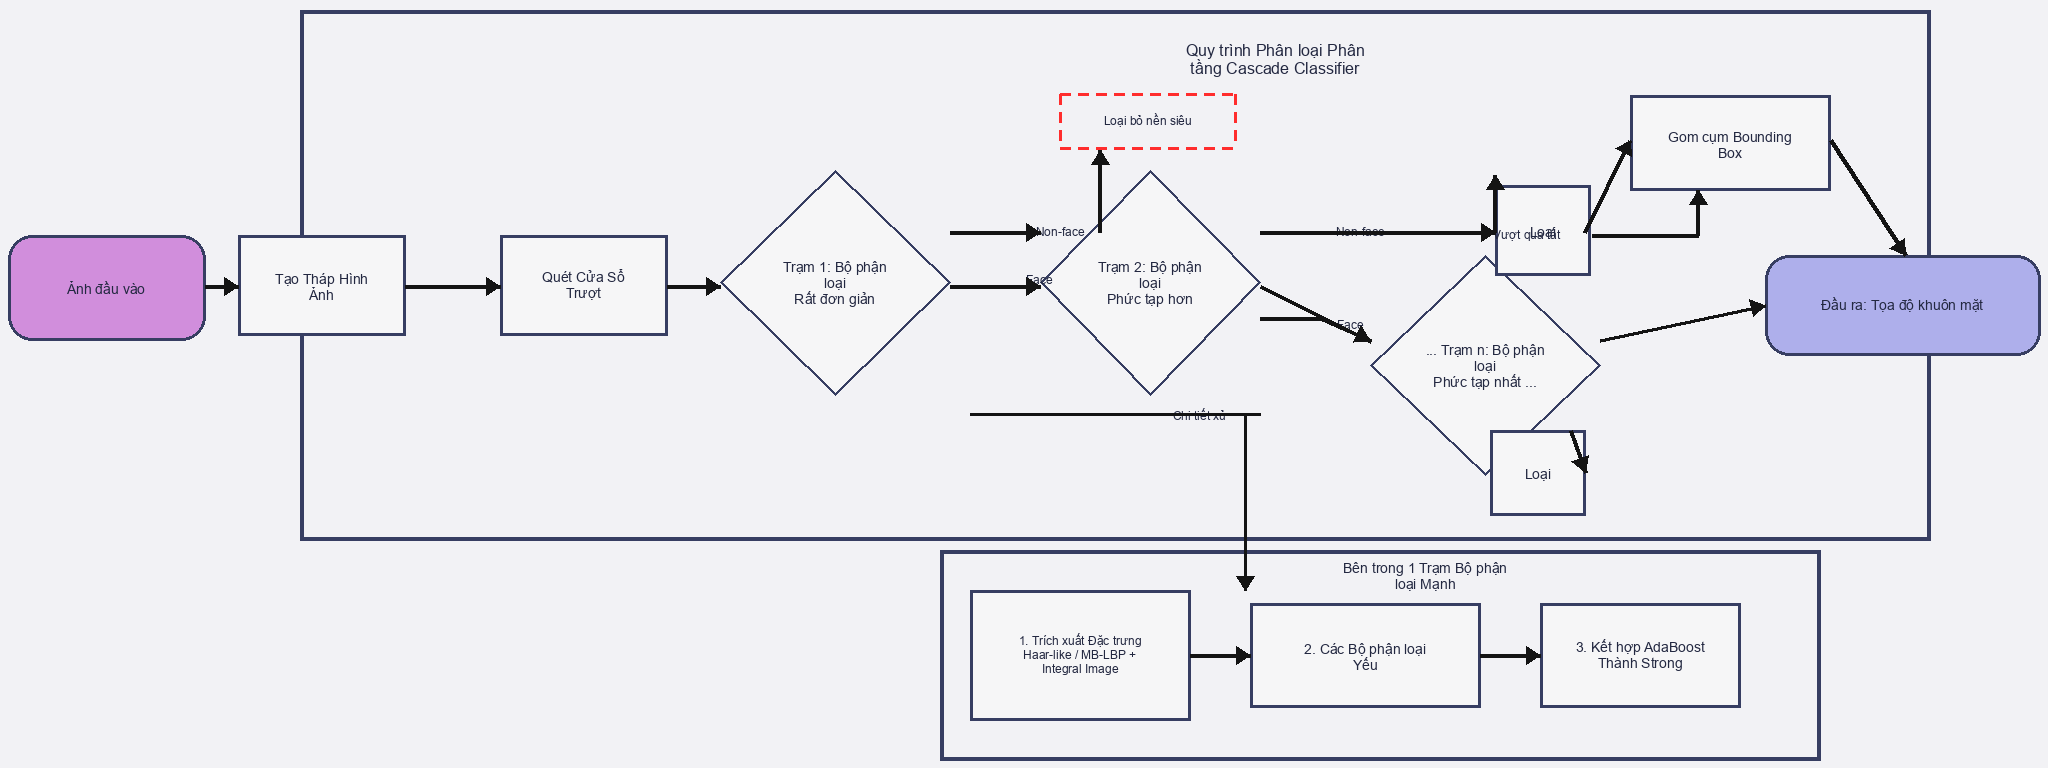
\includegraphics[width=0.92\linewidth]{custom/classical_cascade_detailed_flow.png}
  \end{center}
\end{frame}

\begin{frame}{Minh họa cài đặt: OpenCV Haar Cascade}
  \begin{columns}[T,onlytextwidth]
    \column{0.54\textwidth}
    \begin{itemize}
      \setlength{\itemsep}{5pt}
      \item Dùng \texttt{CascadeClassifier} (OpenCV) với mô hình \texttt{frontalface} mặc định.\ \cite{bradski2000opencv,opencv_cascade_docs}
      \item Quan sát lỗi điển hình:
        \begin{itemize}
          \setlength{\itemsep}{2pt}
          \item khó với khuôn mặt nhỏ/che khuất,
          \item nhạy với góc quay, ánh sáng,
          \item false positive trên nền có cấu trúc tương tự.
        \end{itemize}
    \end{itemize}
    \column{0.46\textwidth}
    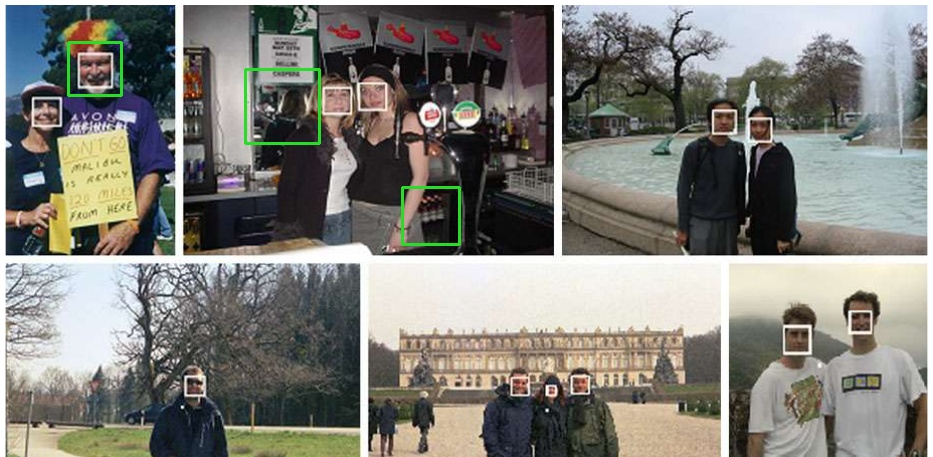
\includegraphics[width=\linewidth]{ch1_classical/book_fig1114_reproduce_final.jpg}
    \vspace{2pt}
    {\scriptsize Ví dụ minh họa (WIDER FACE val).}
  \end{columns}
\end{frame}

\section{Chương II -- Phương pháp bài báo SCRFD (hiện đại)}

\begin{frame}{(2) Phương pháp chính của bài báo: SCRFD}
  \begin{block}{Mục tiêu}
    Tối ưu \textbf{độ chính xác--chi phí tính toán} cho phát hiện khuôn mặt, đặc biệt là \textbf{khuôn mặt nhỏ} trong ảnh độ phân giải thấp (ví dụ VGA).\ \cite{guo2022scrfd}
  \end{block}
  \begin{itemize}
    \setlength{\itemsep}{4pt}
    \item \textbf{Computation Redistribution (CR):} tái phân bổ FLOPs giữa \textit{backbone--neck--head}.
    \item \textbf{Sample Redistribution (SR):} tái phân bổ mẫu dương theo thang tỉ lệ qua tìm kiếm tập scale augmentation.
    \item \textbf{Triển khai:} random search trong search space thiết kế gọn \(\Rightarrow\) tạo ``họ'' SCRFD theo nhiều mức GFLOPs.
  \end{itemize}
\end{frame}

\begin{frame}{Kiến trúc tổng quát (Backbone--Neck--Head)}
  \begin{columns}[T,onlytextwidth]
    \column{0.52\textwidth}
    \begin{itemize}
      \setlength{\itemsep}{5pt}
      \item Nền tảng theo hướng single-shot, có neck đa tỉ lệ và head dự đoán dày đặc.\ \cite{guo2022scrfd}
      \item Điểm nhấn của SCRFD không phải ``module mới'', mà là \textbf{phân bổ đúng tài nguyên} cho đúng nơi cần.
    \end{itemize}
    \column{0.48\textwidth}
    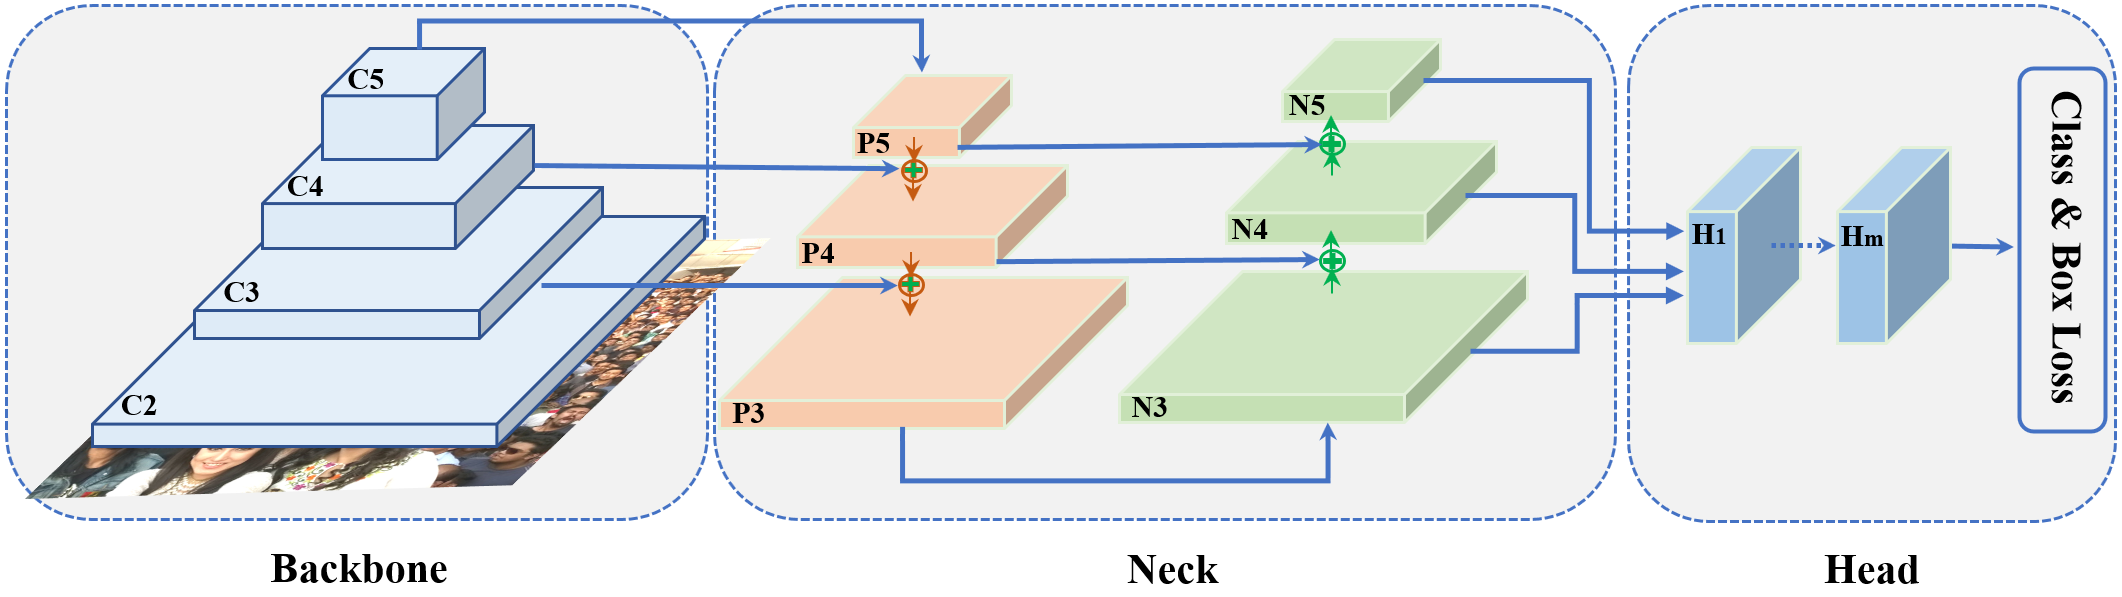
\includegraphics[width=\linewidth]{custom/scrfd_backbone_neck_head.png}
  \end{columns}
\end{frame}

\begin{frame}{Computation Redistribution (CR): ý tưởng và tham số}
  \begin{itemize}
    \setlength{\itemsep}{5pt}
    \item Search space gọn: backbone 4 stage (\(C_2 \rightarrow C_5\)) với \(\{d_i, w_i\}\); neck có \(n\) kênh; head có \(m\) conv và \(h\) kênh.\ \cite{guo2022scrfd}
    \item \textbf{Two-step} (theo paper): tối ưu backbone trước, sau đó tối ưu cả detector để ổn định tỉ lệ FLOPs.
    \item Kết luận thực nghiệm: ưu tiên FLOPs cho backbone (đặc biệt tầng nông) và nén neck/head trong nhiều chế độ compute.
  \end{itemize}
  \vspace{4pt}
  \begin{center}
    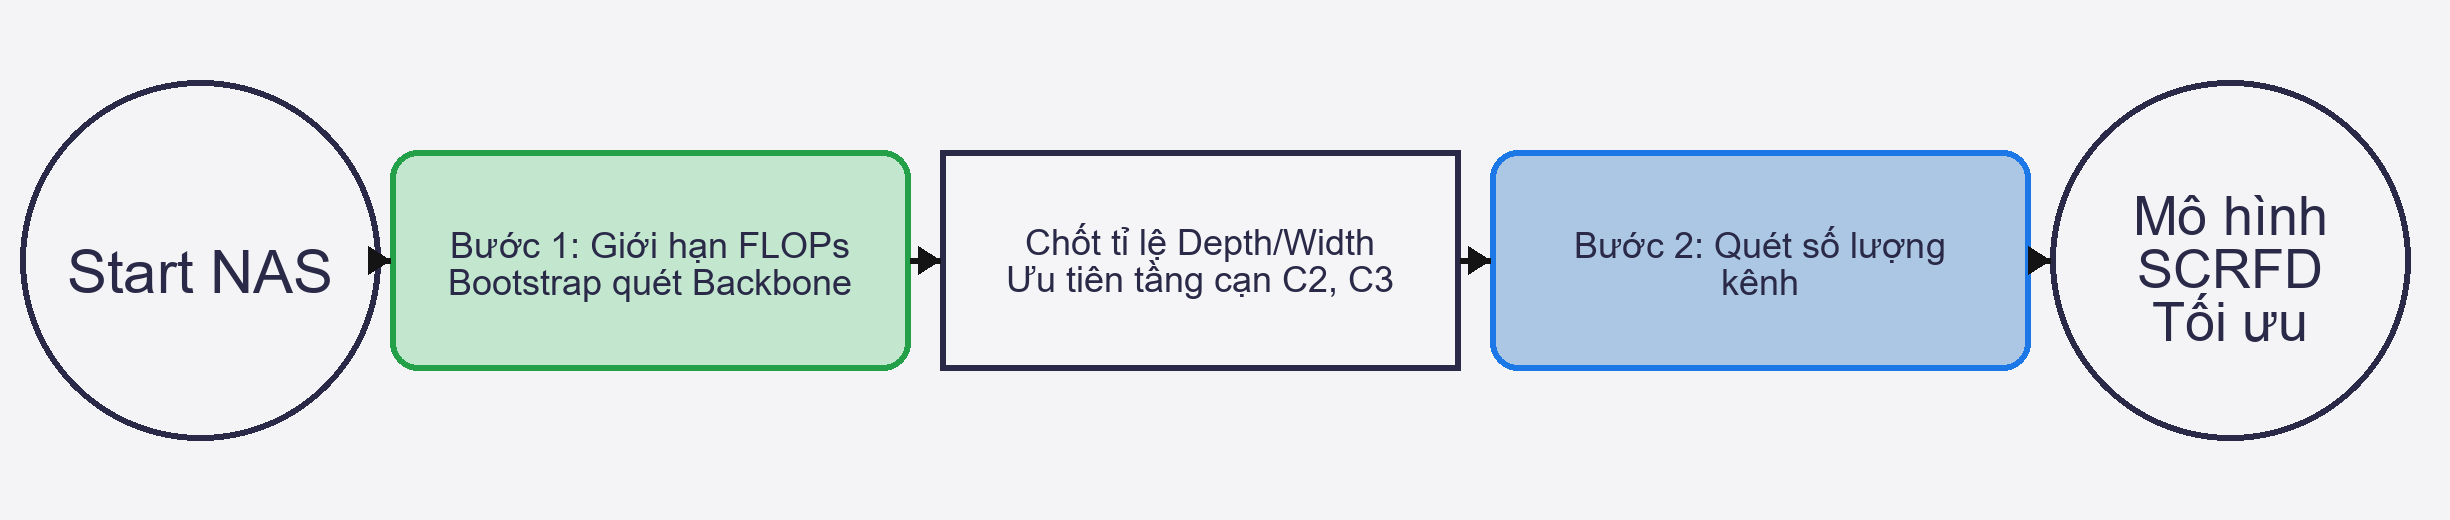
\includegraphics[width=0.88\linewidth]{custom/scrfd_two_step_nas_flow.png}
  \end{center}
\end{frame}

\begin{frame}{Sample Redistribution (SR): tái phân bổ mẫu theo tỉ lệ}
  \begin{itemize}
    \setlength{\itemsep}{5pt}
    \item Quan sát: phát hiện mặt nhỏ phụ thuộc mạnh vào \textbf{phân phối tỉ lệ} và augmentation.\ \cite{guo2022scrfd}
    \item Thiết kế ``zoom-in / zoom-out'' search-able:
      \begin{itemize}
        \setlength{\itemsep}{2pt}
        \item chọn tập scale rời rạc \(S=\{s_{\min}, s_{\min}+0.1, \ldots, s_{\max}\}\),
        \item random search nhiều tập scale \(\Rightarrow\) chọn tập có AP tốt nhất.
      \end{itemize}
    \item Ý nghĩa: tăng xác suất xuất hiện khuôn mặt nhỏ ở các feature map cần thiết.
  \end{itemize}
\end{frame}

\begin{frame}{Kết quả định lượng: trade-off Accuracy--Efficiency}
  \begin{itemize}
    \setlength{\itemsep}{6pt}
    \item SCRFD báo cáo hiệu quả cao trên WIDER FACE; ví dụ SCRFD-34GF hơn TinaFace \(+4.78\%\) AP (hard) và nhanh hơn \(>3\times\) trên GPU (VGA).\ \cite{guo2022scrfd,yang2016widerface}
    \item Ablation (paper): CR và SR đều đóng góp; kết hợp cho cải thiện mạnh nhất ở hard set.\ \cite{guo2022scrfd}
  \end{itemize}
  \vspace{6pt}
  \small
  \begin{tabular}{@{}lccc@{}}
    \toprule
    \textbf{Thiết lập (2.5GF)} & \textbf{Easy} & \textbf{Medium} & \textbf{Hard} \\
    \midrule
    Baseline (ResNet, aug mặc định) & 91.87 & 89.49 & 67.32 \\
    CR@two-steps (CRFD)            & 92.66 & 90.72 & 71.37 \\
    CR@two-steps + SR (SCRFD)      & 93.78 & 92.16 & 77.87 \\
    \bottomrule
  \end{tabular}
  \vspace{2pt}
  {\scriptsize (Bảng rút gọn từ ablation trong paper, tập validation @ VGA).}
\end{frame}

\section{Liên hệ sách--paper và đánh giá}

\begin{frame}{(3) Mối liên hệ giữa chương sách và SCRFD}
  \begin{itemize}
    \setlength{\itemsep}{5pt}
    \item \textbf{Đa tỉ lệ:} tháp ảnh (Viola--Jones) \(\rightarrow\) pyramid feature (CNN/neck) và scale augmentation (SR).\ \cite{li2012facechapter,guo2022scrfd}
    \item \textbf{Tiết kiệm tính toán:} cascade loại sớm theo mức độ khó \(\rightarrow\) CR tái phân bổ FLOPs đúng tầng/cấu phần quan trọng.
    \item \textbf{Khung 3 bước giữ nguyên:} sinh ứng viên / chấm điểm / hợp nhất (NMS) vẫn là xương sống triển khai.
  \end{itemize}
\end{frame}

\begin{frame}{Khác biệt cốt lõi: cổ điển vs nghiên cứu hiện đại}
  \small
  \renewcommand{\arraystretch}{1.15}
  \begin{tabular}{@{}p{0.32\textwidth}p{0.32\textwidth}p{0.32\textwidth}@{}}
    \toprule
    \textbf{Khía cạnh} & \textbf{Chương sách (Viola--Jones)} & \textbf{Paper (SCRFD)} \\
    \midrule
    Đặc trưng & Haar/MB-LBP thủ công & CNN đa tầng học sâu \\
    Tối ưu compute & Cascade loại sớm & CR (FLOPs backbone/neck/head) \\
    Xử lý tỉ lệ & Image pyramid + cửa sổ trượt & FPN/PAFPN + SR (scale search) \\
    Thiết kế hệ & Rule-based + boosting & Data-driven + random/NAS search \\
    \bottomrule
  \end{tabular}
\end{frame}

\begin{frame}{(4) Đánh giá kỹ thuật: điểm mạnh, hạn chế, phạm vi}
  \begin{columns}[T,onlytextwidth]
    \column{0.5\textwidth}
    \textbf{Điểm mạnh (SCRFD)}
    \begin{itemize}
      \setlength{\itemsep}{4pt}
      \item Hiệu quả ở nhiều mức compute, đặc biệt ảnh low-res.\ \cite{guo2022scrfd}
      \item Thiết kế ``đúng prior'' của khuôn mặt \(\Rightarrow\) tránh dư thừa như detector tổng quát.
      \item CR/SR đơn giản, có thể áp dụng như quy trình tối ưu.
    \end{itemize}
    \column{0.5\textwidth}
    \textbf{Hạn chế / giả định}
    \begin{itemize}
      \setlength{\itemsep}{4pt}
      \item Phụ thuộc phân phối dữ liệu (WIDER FACE) và chiến lược augmentation.\ \cite{yang2016widerface}
      \item Random search/NAS tốn chi phí huấn luyện; tái lập đầy đủ cần tài nguyên.
      \item Vẫn cần NMS; độ bền với domain shift/occlusion cần kiểm chứng thêm.
    \end{itemize}
  \end{columns}
\end{frame}

\begin{frame}{(5) Nhận định cá nhân và hướng mở rộng}
  \begin{itemize}
    \setlength{\itemsep}{6pt}
    \item \textbf{Nhận định:} SCRFD cho thấy ``tối ưu đúng chỗ'' (CR/SR) có thể đem lại bước nhảy lớn về trade-off mà không cần kiến trúc phức tạp.
    \item \textbf{Hướng mở rộng khả thi:}
      \begin{itemize}
        \setlength{\itemsep}{3pt}
        \item distillation cho các bản 0.5--1.0GF để giữ AP khi ràng buộc compute,
        \item hardware-aware search (CPU/mobile NPU) thay vì chỉ GFLOPs,
        \item cải thiện robustness (che khuất, ánh sáng) bằng dữ liệu/augmentation mục tiêu.
      \end{itemize}
  \end{itemize}
\end{frame}

\section{Chuẩn học thuật và tài liệu tham khảo}

\begin{frame}{(6) Trình bày học thuật và liêm chính}
  \begin{itemize}
    \setlength{\itemsep}{6pt}
    \item Mọi số liệu/kết luận định lượng đều gắn nguồn (paper/dataset).
    \item Hình minh họa tự tạo (pipeline) hoặc trích dẫn theo tài liệu gốc; tránh sao chép không ghi nguồn.
    \item Có thể đối chiếu: chương sách \cite{li2012facechapter}, paper \cite{guo2022scrfd}, WIDER FACE \cite{yang2016widerface}, OpenCV \cite{bradski2000opencv,opencv_cascade_docs}.
  \end{itemize}
\end{frame}

\begin{frame}[allowframebreaks]{Tài liệu tham khảo}
  \ifhascites
    \printbibliography
  \else
    {\small (Chưa có trích dẫn trong slide.)}
  \fi
\end{frame}

\begin{frame}{Q\&A}
  \centering
  \Large Cảm ơn thầy/cô và các bạn!
\end{frame}

\end{document}
